\documentclass[journal]{IEEEtran}
\usepackage{amssymb}
\usepackage{amsmath}
\usepackage[colorlinks=true, linkcolor=black]{hyperref} % Links
\usepackage{makeidx} % Indexierung
\usepackage{siunitx}
%\usepackage[ngerman]{babel} % deutsche Sonderzeichen
\usepackage[utf8]{inputenc}
\usepackage{geometry} % Dokumentendesign wie Seiten- oder Zeilenabstand bestimmen
\usepackage{algorithm}
\usepackage{algorithmic}
\usepackage{caption}
\usepackage{subcaption}
%\usepackage[toc,page]{appendix}

% Graphiken
\usepackage{tikz}
\usepackage{pgfplots}
\usepackage{pgfmath}
\usepackage{pgfcore}
\usepackage{pgfopts}
\usepackage{pgfkeys}
\usepackage{pgfornament}
\usepackage{pgf}
\usepackage{ifthen}
\usepackage{booktabs}

% Tabellen
\usepackage{tabu}
\usepackage{longtable}
\usepackage{colortbl} % Tabellen faerben
\usepackage{multirow}
\usepackage{diagbox} % Tabellenzelle diagonal splitten

\usepackage{xcolor} % Farben
\usepackage[framemethod=tikz]{mdframed} % Hintergrunderstellung
\usepackage{enumitem} % Enumerate mit Buchstaben nummerierbar machen
\usepackage{pdfpages}
\usepackage{listings} % Source-Code darstellen
\usepackage{eurosym} % Eurosymbol
\usepackage[square,numbers]{natbib}
\usepackage{here} % figure an richtiger Stelle positionieren
\usepackage{verbatim} % Blockkommentare mit \begin{comment}...\end{comment}
\usepackage{ulem} % \sout{} (durchgestrichener Text)
\usepackage{abstract}
\usepackage{blindtext}
\usepackage{fancyref}

% BibLaTex
\bibliographystyle{acm}

% Aendern des Anhangnamens (Seite und Inhaltsverzeichnis)
%\renewcommand\appendixtocname{Anhang}
%\renewcommand\appendixpagename{Anhang}

% mdframed Style {{{
\mdfdefinestyle{codebox}{
	linewidth=2.5pt,
	linecolor=codebordercolor,
	backgroundcolor=codecolor,
	shadow=true,
	shadowcolor=black!40!white,
	fontcolor=black,
	everyline=true,
}
% }}}

% Seitenabstaende
%\geometry{left=15mm,right=15mm,top=15mm,bottom=20mm}

% TikZ Bibliotheken {{{
\usetikzlibrary{
    arrows,
    arrows.meta,
    decorations,
    backgrounds,
    external,
    positioning,
    fit,
    petri,
    shadows,
    datavisualization.formats.functions,
    calc,
    shapes,
    shapes.multipart,
    matrix
}
% }}}

\pgfplotsset{width=7cm,compat=1.15}

\definecolor{codecolor}{HTML}{EEEEEE}
\definecolor{codebordercolor}{HTML}{CCCCCC}

% Standardeinstellungen fuer Source-Code listings {{{
\lstset{
    language=C,
    breaklines=true,
    keepspaces=true,
    keywordstyle=\bfseries\color{green!70!black},
    basicstyle=\ttfamily\color{black},
    commentstyle=\itshape\color{purple},
    identifierstyle=\color{blue},
    stringstyle=\color{orange},
    showstringspaces=false,
    rulecolor=\color{black},
    tabsize=2,
    escapeinside={\%*}{*\%},
}
% }}}

%\input{libuml}
%\input{liberm}

\title{Partial Classification Forest}

\author{Jonas Fa{\ss}bender \\ [1ex]
  \href{mailto: jonas@fc-web.de}{jonas@fc-web.de}}
\date{}

\begin{document}

\maketitle

\begin{abstract}
  %\noindent  \blindtext
\end{abstract}

\section{Introduction}
\label{sec:intro}

Some datasets do not allow a classifier to generate a
decision surface good enough to be able to predict unseen
observations well. A dataset contains tuples of
observations and their labels. An observation is a point
inside the feature space whereas the label is an element
from a finite set called label set. A classification
problem is the goal to find a function that maps the
feature space to the label space based on the observations
and their respective labels provided by the dataset.%
\cite[chapter 18]{ki} This function is called a classifier.

Sometimes a classifier needs to fulfill a certain quality
criteria in order to consider it a solution to the
respective classification problem. For example: think of
any classification problem that needs a classifier to have
an accuracy of 99 percent --- in this case impossible to
find for the given dataset.

For some of those classification problems it may still be
valuable to predict only on partitions of the feature
space if the problem is partially solvable. A
classification problem is partially solvable if a
classifier can return the label of an observation or
nothing if it is not certain enough it can predict the
correct label. Non-partial classifier always return a
label.

For the example above: if there exists at least one
partition of the feature space in which a classifier can be
found that has an accuracy of 99 percent the problem still
can be partially solved if this is desired.

More generally accuracy would be the quality metric,
the classifier's accuracy is the quality measurement and 99
percent is the quality threshold which must be met by a
classifier's quality measurement in order to consider the
classifier a (partial) solution to the classification
problem. Any metric --- for example a loss metric -- can be
used to determine a classifier's quality.

I call this concept Partial Classification. The idea
opposes the classical, non-partial approach. The
non-partial approach would be trying to increase a
classifier's quality until it equals or exceeds the quality
threshold. Partial Classification takes the other way
around. A partial classifier takes the quality threshold as
its input and tries to find partitions of the feature space
in which it can reach the quality. So rather than
increasing the quality of the classifier the goal in
Partial Classification is to increase the (sub-)space in
which a partial classifier can predict.

This paper proposes a Monte Carlo based ensemble method
realizing Partial Classification called Partial
Classification Forest (PCF). The PCF builds an ensemble of
trees having a structure similar to k-d trees. An instance
of this tree structure partitions the feature space of a
given dataset in order to find partitions, making Partial
Classification possible.

It should be noted here: this paper is rather a Proof
of Concept describing the structures and algorithms of a
very early version of the PCF. It has several shortcomings
in research and empirical tests, due to a lack of time and
no complete, fast implementation. These shortcomings are:

\begin{itemize}

\item Tests with a more sophisticated $\gamma$ (see
      Section~\ref{subsec:fit})

\item The PCF's performance on high dimensional data

\item Untested possible optimizations and features (see
      Section~\ref{sec:features})

\item A Tree's growing behavior

\item Benchmarks

\end{itemize}

In Section~\ref{sec:tree} I will lay out
the structure and the operations of the k-d tree like
structure the PCF uses.

In this paper such a tree generated by the PCF is
spelled Tree --- with a capital T --- rather than tree,
which is used to denote the tree data structure.

In Section~\ref{sec:pcf} I will describe how the PCF works
and utilizes Tree instances. After that I will continue
displaying the application of the PCF and compare it to
other, non-partial classifiers.

Because this paper is concerned with an early version of
the PCF it will also contain a discussion about possible
additional features which could further increase the PCF's
performance in Section~\ref{sec:features}.

Last I will finish with my conclusions and a road map.


\section{The Tree structure}
\label{sec:tree}

A Tree generated by the PCF is an instance of a binary
search tree structure similar to the k-d tree.
Its purpose is to randomly generate disjoint partitions of
the feature space of a given dataset.

A Tree has two types of nodes: non-leaf nodes --- here
denoted as (\romannumeral 1) Nodes --- and leaf nodes
denoted as  (\romannumeral 2) Leaves. It provides two
operations: (\romannumeral 1) FIT, initializing the Tree
and (\romannumeral 2) PREDICT, returning a label for an
observation or $\Lambda$ if uncertain.

The Node structure contains three properties:
(\romannumeral 1) a split value; (\romannumeral 2) a left
and (\romannumeral 3) a right successor, both references to
either another Node or a Leaf.

A Leaf on the other hand is the structure representing a
partition of the feature space, having the following
properties: (\romannumeral 1) $active$: a boolean value
deciding whether the partition' quality --- determined
during the FIT operation --- equals or exceeds the
defined quality threshold; (\romannumeral 2) optionally a
classifier which is used to classify observations during
the PREDICT operation. Only if a Leaf's $active$ property
is true, a classifier must be provided. A Leaf also has two
vectors with arbitrary length as properties:
(\romannumeral 3) a vector containing the observations of
the dataset used in FIT, which are laying inside the
partition and (\romannumeral 4) their inherent labels.

During the FIT operation a Tree contains a third type of
node, Nil. Nil is used to initialize Trees
and the left and right successor of a Node. These nodes are
transformed during FIT to either a Node or a Leaf, so after
the FIT operation a Tree does not contain Nil nodes
anymore. A Nil node does not have any properties.

\subsection{The FIT operation}
\label{subsec:fit}

The FIT operation constructs a Tree based on a dataset
split into observations ($X$) and their labels ($y$).
Algorithm~\ref{alg:fit} shows how FIT recursively builds a
Tree from a pointer to a Nil node.

The most important parameter passed to FIT is $\gamma$.
$\gamma$ is a function returning (\romannumeral 1) a
classifier and (\romannumeral 2) the loss of it. Otherwise
$\gamma$ is treated as a black box by the PCF, so what the
classifier is and how its loss is calculated are not
relevant to the PCF, as long as the classifier is callable%
\footnote{There could be another interface for the
  classifier, for example a predict method similar to the
  scikit-learn library.\cite{sklearn_api}}
and returns an element from the label set when being
called (Algorithm~\ref{alg:pred}, line 9). The loss
returned by $\gamma$ gets compared to the quality threshold
$\tau_l$. Is the loss $\leq \tau_l$ the classifier returned
by $\gamma$ is considered good enough and $\Theta$ is
transformed into an active Leaf (Algorithm~\ref{alg:fit},
lines 2, 3).

There are two other thresholds besides $\tau_l$:
$\tau_{|X|}$ and $\tau_h$. Both regulate the behavior of a
Tree's growth. $\tau_{|X|}$ defines a minimum amount of
observations a Leaf must contain. Without $\tau_{|X|}$ or
$\tau_{|X|} = 0$ a Tree would never stop growing, since FIT
would continue to split empty partitions trying to find a
smaller partition which could be predictable, even though
no classifier can be generated without observations to
train it on.

$\tau_h$ further regulates the maximum path length of a
Tree. It is necessary besides $\tau_{|X|}$: be
$\tau_{|X|} = 2$ and there are two equal observations in
the dataset, both having a different label than the other
one. $\gamma$---passed $X$ containing only those two
identical observations---returns a classifier with a
loss $> \tau_l$. Since $|X|$ is still not smaller than
$\tau_{|X|}$ FIT would continue trying to separate the two
inseparable observations. To prevent such a scenario
$\tau_h$ regulates FIT to stop before the Tree's height%
---the amount of edges of the longest path---would
exceed $\tau_h$. The path length of the Tree's root to
$\Theta$ is passed as a parameter $h$ to FIT. $\tau_h$ also
provides a way to further regulate the time complexity of
FIT and PREDICT.

FIT performs a split and transforms $\Theta$ to a Node
(Algorithm~\ref{alg:fit}, lines 7ff), if neither the
classifier's loss matches $\tau_l$ nor $\tau{|X|}$ or
$\tau_h$ is violated. The dimension the split is performed
on is chosen in a cyclic manner, a practice also applied to
k-d trees (Algorithm~\ref{alg:fit}, line 7).%
\cite{Brown2015kdtree}
But rather than choosing the splitting value at the median
of the observations in the dimension---done in order to
construct balanced k-d trees---the splitting value
is determined randomly.\cite{Brown2015kdtree}

In order to chose a proper splitting value $\beta_X$ is
passed as another parameter to FIT. $\beta_X$ represents
the boundaries for every dimension of the feature space
based on $X$. For each dimension $\beta_X$ contains a
tuple with the minimum and maximum value in the dimension
of all observations in $X$.

$\beta_X[\text{dimension}]$ is passed to a pseudo-random
number generator\footnote{The implementation used in
  Section~\ref{sec:application} utilizes Python 3.6's
  random library.\cite[chapter 9.6]{python}}
generating a random value so that
$lower(\beta_X[\text{dimension}]) \leq \text{random number}
\leq upper(\beta_X[\text{dimension}])$
(Algorithm~\ref{alg:fit}, line 8).

Afterwards $X$, $y$, $\beta_X$ are split into two new
disjoint partitions and FIT is recursively applied to both
(Algorithm~\ref{alg:fit}, lines 10ff).

Since $\tau_h$ is defined, the maximum amount of nodes a
Tree can have is $2^{\tau_h + 1} - 1$, if the Tree is
perfectly balanced.\cite[chapter 16.1]{Teschl} For each
node FIT is called, so building a Tree has a worst case
time complexity of:
\begin{align}
  \mathcal{O}((2^{\tau_h + 1} -1)*\mathcal{O}(\text{FIT})).
\end{align}
$\mathcal{O}(\text{FIT})$ is determined by the size of $X$%
---since $X$ has to be iterated in order to split it---and
by $\mathcal{O}(\gamma)$. That said, a single FIT
operation would have a worst case time complexity of:
\begin{align}
  \mathcal{O}(|X| + \mathcal{O}(\gamma)),
\end{align} which means the time complexity of the whole
fitting process is:
\begin{align}
  \mathcal{O}((2^{\tau_h + 1} - 1) *
  (|X| + \mathcal{O}(\gamma)))
\label{eq:O_fit}
\end{align}

% algorithm {{{
\begin{algorithm}
  \caption{: FIT($\Theta, X, y, h, \beta_X, \gamma,
    \tau_{l}, \tau_{|X|}, \tau_{h}$)}%
  \label{alg:fit}
  A Tree's FIT operation.

  Inputs:

    \begin{tabu}{llX}
    $\Theta$ &$-$ &a pointer to a Nil node; initially
      pointing to the root node of an empty Tree,\\
    $X$ &$-$ &input data,\\
    $y$ &$-$ &labels of X,\\
    $h$ &$-$ &height of the Tree; initially $h = 0$,\\
    $\beta_X$ &$-$ &lower and upper boundaries of every
      dimension of X,\\
    $\gamma$ &$-$ &function returning a classifier and its
      loss,\\
    $\tau_{l}$ &$-$ &loss threshold,\\
    $\tau_{|X|}$ &$-$ &threshold for the size of X,\\
    $\tau_{h}$ &$-$ &height limit of the Tree
    \end{tabu}

  Output: void

  \noindent\rule{\linewidth}{0.4pt}

  \begin{algorithmic}[1]
    \STATE classifier, loss $\leftarrow \gamma(X, y)$
    \IF{loss $\leq \tau_{l}$}
      \STATE $\Theta \leftarrow$ LEAF(\TRUE, classifier,
         $X$, $y$)
    \ELSIF{$h > \tau_{h}$ \OR $|X| < \tau_{|X|}$ \OR
        loss $> \tau_{l}$}
      \STATE $\Theta \leftarrow$ LEAF(\FALSE, classifier,
        $X$, $y$)
    \ELSE
      \STATE dimension $\leftarrow h$ mod $|X[0]|$
      \STATE split $\leftarrow$ RANDOM($\beta_X[
        \text{dimension}]$)
      \STATE $\Theta \leftarrow$ NODE(split, NIL, NIL)
      \STATE split $X$, $y$ and $\beta_X$ into
        $X'$, $X''$, $y'$, $y''$, $\beta_X'$, $\beta_X''$
      \STATE FIT($\Theta$.left, $X'$, $y'$, $h + 1$,
        $\beta_X'$, \dots)
      \STATE FIT($\Theta$.right, $X''$, $y''$, $h + 1$,
        $\beta_X''$, \dots)
    \ENDIF
  \end{algorithmic}
\end{algorithm}
% }}}

\begin{figure*}
  \begin{subfigure}[b]{\textwidth}
    \centering
    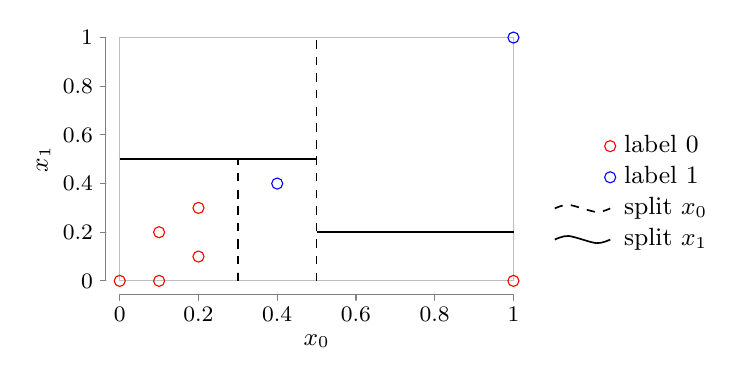
\begin{tikzpicture}
  \datavisualization[
    scientific axes = clean,
    x axis={label={$x_0$}},
    y axis={label={$x_1$}},
    visualize as smooth line/.list={
      split0,split1,split2,split3
    },
    visualize as scatter/.list={0,1},
    0={label in legend={text=label 0},
      style={mark=o, visualizer color=red}},
    1={label in legend={text=label 1},
      style={mark=o, visualizer color=blue}},
    split0={label in legend={text=split $x_0$},
      style={dashed}},
    split1={label in legend={text=split $x_1$}},
    split3={style={dashed}},
  ]
  data {
    x,  y,  set
    0,  0,  0
    0.1,0,  0
    0.2,0.1,0
    0.2,0.3,0
    0.1,0.2,0
    1,  0,  0
    0.4,0.4,1
    1,  1,  1
    0.5,0,  split0
    0.5,1,  split0
    0,  0.5,split1
    0.5,0.5,split1
    0.5,0.2,split2
    1,  0.2,split2
    0.3,0,  split3
    0.3,0.5,split3
  };
\end{tikzpicture}

    \caption{Scatterplot showing the observations and the
      splits done by the FIT operation.}
    \label{fig:scatter_example}
  \end{subfigure}
  \begin{subfigure}[b]{\textwidth}
    \centering
    \scalebox{0.9}{\def\Node#1#2{
  \node[
    rectangle split,
    rectangle split parts=3,
    rectangle split horizontal,
    draw
  ] (#1) {#2\nodepart{two}\nodepart{three}};
}
\def\NodeR#1#2#3{
  \node[
    rectangle split,
    rectangle split parts=3,
    rectangle split horizontal,
    draw,
    #3
  ] (#1) {#2};
}
\def\LeafR#1#2#3{
  \node[
    rectangle split,
    rectangle split parts=3,
    rectangle split horizontal,
    rounded corners,
    draw,
    #3
   ] (#1) {#2};
}
\def\l#1#2{
  \draw[->] ($(#1.two split)!.5!(#1.text split)$)
    |- ($(#1.south)!.5!(#2.north)$) -| (#2.north);
}
\def\r#1#2{
  \draw[->] ($(#1.two split)!.5!(#1.east)$)
    |- ($(#1.south)!.5!(#2.north)$) -| (#2.north);
}
\def\D#1#2#3{
  \matrix[
    ampersand replacement=\&,
    matrix of nodes,
    left delimiter={[},
    right delimiter={]},
    outer ysep=3pt,
    #2
  ] (#1) {#3};
}

\begin{tikzpicture}[
  every left delimiter/.style={xshift=2ex},
  every right delimiter/.style={xshift=-2ex},
]
  % for margin
  \node at(0,1) {};

  \Node{root}{0.5}
    \NodeR{al}{0.5}{below left=0.5 and 2 of root}
      \NodeR{bl}{0.3}{below left=0.5 of al}
        \LeafR{lb}{true}{below left=0.5 and 0.1 of bl}
          \D{lbx}{below left=0.5 and -.75 of lb} {
            0   \& 0   \\
            0.1 \& 0   \\
            0.2 \& 0.1 \\
            0.2 \& 0.3 \\
            0.1 \& 0.2 \\
          }
          \D{lby}{below right=0.5 and .15 of lb} {
            0 \\
            0 \\
            0 \\
            0 \\
            0 \\
          }
        \LeafR{lc}{false}{below right=.5 and 0.1 of bl}
          \D{lcx}{below left=0.5 and -.75 of lc} {
            0.4 \& 0.4 \\
          }
          \D{lcy}{below right=.5 and .15 of lc}{
            1 \\
          }
      \LeafR{la}{false}{below right=0.5 of al}
        \D{lax}{below left=.3 and -.75 of la}{
          \textcolor{white}{1} \&
          \textcolor{white}{1}\\
        }
        \D{lay}{below right=.3 and .15 of la}{
          \textcolor{white}{1}\\
        }
    \NodeR{ar}{0.2}{below right=0.5 and 2 of root}
      \LeafR{ld}{false}{below left=0.5 of ar}
        \D{ldx}{below left=.3 and -.75 of ld} {
          1 \& 0 \\
        }
        \D{ldy}{below right=.3 and .15 of ld} {0 \\}
      \LeafR{le}{false}{below right=0.5 of ar}
        \D{lex}{below left=.3 and -.75 of le} {
          1 \& 1 \\
        }
        \D{ley}{below right=.3 and .15 of le} {1 \\}

  \l{root}{al}
    \l{al}{bl}
      \l{bl}{lb}
        \l{lb}{lbx}
        \r{lb}{lby}
      \r{bl}{lc}
        \l{lc}{lcx}
        \r{lc}{lcy}
    \r{al}{la}
      \l{la}{lax}
      \r{la}{lay}
  \r{root}{ar}
    \l{ar}{ld}
      \l{ld}{ldx}
      \r{ld}{ldy}
    \r{ar}{le}
      \l{le}{lex}
      \r{le}{ley}

  \node[
    rectangle split,
    rectangle split parts=3,
    rectangle split horizontal,
    draw,
    below=3.5 of ar
  ] (nd) {};
  \node[right] at (nd.east) {Node};

  \node[
    rectangle split,
    rectangle split parts=3,
    rectangle split horizontal,
    rounded corners,
    draw,
    below=.5 of nd
   ] (lf) {};
   \node[right] at (lf.east) {Leaf};
\end{tikzpicture}
}
    \caption{The structure of the Tree generated by FIT.}
    \label{fig:tree_example}
  \end{subfigure}
  \caption{Example of FIT applied to the dataset seen in
    Figure~\ref{fig:scatter_example}. $\gamma$ simply
    computes the probability of each label in $y$ and
    returns a function returning the label with the
    maximum probability and as loss one minus the maximum
    probability. The thresholds are: $\tau_l = 1$,
    $\tau_{|X|} = 2$. $\tau_h$ can be any integer above
    2.
  }
  \label{fig:fit_example}
\end{figure*}


\subsection{The PREDICT operation}

The PREDICT operation traverses a Tree until it encounters
a Leaf. If the Leaf is active a label to a provided
observation $x$ is returned by the predictor
property of the Leaf, otherwise $\Lambda$ is returned.

$\Lambda$ must not be an element of the label set.

\begin{algorithm}
  \caption{: PREDICT($\Theta, x, h$)}%
  \label{alg:pred}
  Inputs:

    \begin{tabu}{llX}
    $\Theta$ &$-$ &a Tree node; initially pointing to the
      root of the Tree,\\
    $x$ &$-$ &an observation,\\
    $h$ &$-$ &height of the Tree; initially $h = 0$
    \end{tabu}

  Output: the predicted label or $\Lambda$

  \noindent\rule{\linewidth}{0.4pt}

  \begin{algorithmic}[1]
    \IF{TYPE($\Theta$) is Node}
      \STATE dimension $\leftarrow h$ mod $|x|$
      \IF{$x[dimension] \leq \Theta$.split}
        \STATE PREDICT($\Theta$.left, $x$, $h + 1$)
      \ELSE
        \STATE PREDICT($\Theta$.right, $x$, $h + 1$)
      \ENDIF
    \ELSIF{$\Theta$.active}
      \RETURN $\Theta$.predictor($x$)
    \ELSE
      \RETURN $\Lambda$
    \ENDIF
  \end{algorithmic}
\end{algorithm}



\section{Partial Classification Forest}
\label{sec:pcf}

The PCF has two parameters, (\romannumeral 1) $N$ and
(\romannumeral 2) an array with $N$ pointers.
$N$ is the amount of Trees the PCF maintains.
Initially the pointers inside the array are references to
Nil nodes.

The PCF offers the same two operations a Tree has, FIT
(Algorithm~\ref{alg:pcf_fit}) and PREDICT (Algorithm~%
\ref{alg:pcf_pred}), both abstractions to the equivalent
Tree operations.

Once FIT is executed, the pointers are references to the
roots of fitted Tree instances.

Both FIT and PREDICT can be implemented as multi-threaded
operations as long as $\gamma$ is thread-safe, since the
Tree instances are independent of each other and the shared
parameters $X$, $y$ (FIT) and $x$ (PREDICT) are read only,
making synchronization unnecessary.

FIT first computes $\beta_X$ which has a time complexity
of:
\begin{align}
  \mathcal{O}(|\text{dimensions}(X)| * |X|).
\end{align}

After that the Tree's FIT operation is called $N$ times,
which means the PCF's FIT operation has a worst case time
complexity of:
\begin{align}
  \mathcal{O} (N * \text{FIT} + |\text{dimensions}(X)|*|X|)
\end{align}
(see Equation~\ref{eq:O_fit} for $\mathcal{O}$(FIT)).

% {{{
\begin{algorithm}
  \caption{: FIT($\Pi, X, y, \gamma, \tau_{l},
    \tau_{|X|}, \tau_{h}$)}%
  \label{alg:pcf_fit}
  The PCF's FIT operation.

  Inputs:

    \begin{tabu}{llX}
    $\Pi$ &$-$ &a PCF instance,\\
    $X$ &$-$ &input data,\\
    $y$ &$-$ &labels of X,\\
    $\gamma$ &$-$ &function returning a classifier and its
      loss,\\
    $\tau_{l}$ &$-$ &loss threshold,\\
    $\tau_{|X|}$ &$-$ &threshold for the size of X,\\
    $\tau_{h}$ &$-$ &height limit of the Tree
    \end{tabu}

  Output: void

  \noindent\rule{\linewidth}{0.4pt}

  \begin{algorithmic}[1]
    \STATE compute $\beta_X$
    \FORALL{$\Theta \in \Pi$.trees}
      \STATE{FIT($\Theta$, $X$, $y$, 0, $\beta_X$, \dots)}
    \ENDFOR
  \end{algorithmic}
\end{algorithm}
% }}}

The PCF's PREDICT operation first initializes an array with
$N$ elements (Algorithm~\ref{alg:pcf_pred}, line 1). Each
Tree instance fills one element of the array with its
prediction. After that the PCF's PREDICT operation takes
the label predicted most and returns it as its prediction
for the observation $x$ (Algorithm~\ref{alg:pcf_pred},
lines 5, 6).

The worst case time complexity of the PCF's PREDICT
operation is:
\begin{align}
  \mathcal{O}(N * (\tau_h + \mathcal{O} (\text{classifier})) + N),
\end{align}
since a Tree's PREDICT operation
is executed $N$ times, plus the most predicted label
must be determined, which is $\mathcal{O}(N)$.

% {{{
\begin{algorithm}
  \caption{: PREDICT($\Pi, x$)}
  \label{alg:pcf_pred}
  The PCF's PREDICT operation.

  Inputs:

    \begin{tabu}{llX}
    $\Pi$ &$-$ &a PCF instance,\\
    $x$ &$-$ &an observation, \\
    \end{tabu}

  Output: the predicted label or $\Lambda$

  \noindent\rule{\linewidth}{0.4pt}

  \begin{algorithmic}[1]
    \STATE predictions $\leftarrow [\Lambda; N]$
    \FOR{$i = 1$ \TO $N$}
      \STATE{predictions$[i]$ = PREDICT($\Pi$.trees$[i]$,
        $x$, $0$)}
    \ENDFOR
    \STATE determine $l_{max}$, the label predicted most
    \RETURN $l_{max}$
  \end{algorithmic}
\end{algorithm}
% }}}


\section{The Tree structure}
\label{sec:tree}

A Tree generated by the PCF is an instance of a binary
search tree structure similar to the k-d tree.
Its purpose is to randomly generate disjoint partitions of
the feature space of a given dataset.

A Tree has two types of nodes: non-leaf nodes --- here
denoted as (\romannumeral 1) Nodes --- and leaf nodes
denoted as  (\romannumeral 2) Leaves. It provides two
operations: (\romannumeral 1) FIT, initializing the Tree
and (\romannumeral 2) PREDICT, returning a label for an
observation or $\Lambda$ if uncertain.

The Node structure contains three properties:
(\romannumeral 1) a split value; (\romannumeral 2) a left
and (\romannumeral 3) a right successor, both references to
either another Node or a Leaf.

A Leaf on the other hand is the structure representing a
partition of the feature space, having the following
properties: (\romannumeral 1) $active$: a boolean value
deciding whether the partition' quality --- determined
during the FIT operation --- equals or exceeds the
defined quality threshold; (\romannumeral 2) optionally a
classifier which is used to classify observations during
the PREDICT operation. Only if a Leaf's $active$ property
is true, a classifier must be provided. A Leaf also has two
vectors with arbitrary length as properties:
(\romannumeral 3) a vector containing the observations of
the dataset used in FIT, which are laying inside the
partition and (\romannumeral 4) their inherent labels.

During the FIT operation a Tree contains a third type of
node, Nil. Nil is used to initialize Trees
and the left and right successor of a Node. These nodes are
transformed during FIT to either a Node or a Leaf, so after
the FIT operation a Tree does not contain Nil nodes
anymore. A Nil node does not have any properties.

\subsection{The FIT operation}
\label{subsec:fit}

The FIT operation constructs a Tree based on a dataset
split into observations ($X$) and their labels ($y$).
Algorithm~\ref{alg:fit} shows how FIT recursively builds a
Tree from a pointer to a Nil node.

The most important parameter passed to FIT is $\gamma$.
$\gamma$ is a function returning (\romannumeral 1) a
classifier and (\romannumeral 2) the loss of it. Otherwise
$\gamma$ is treated as a black box by the PCF, so what the
classifier is and how its loss is calculated are not
relevant to the PCF, as long as the classifier is callable%
\footnote{There could be another interface for the
  classifier, for example a predict method similar to the
  scikit-learn library.\cite{sklearn_api}}
and returns an element from the label set when being
called (Algorithm~\ref{alg:pred}, line 9). The loss
returned by $\gamma$ gets compared to the quality threshold
$\tau_l$. Is the loss $\leq \tau_l$ the classifier returned
by $\gamma$ is considered good enough and $\Theta$ is
transformed into an active Leaf (Algorithm~\ref{alg:fit},
lines 2, 3).

There are two other thresholds besides $\tau_l$:
$\tau_{|X|}$ and $\tau_h$. Both regulate the behavior of a
Tree's growth. $\tau_{|X|}$ defines a minimum amount of
observations a Leaf must contain. Without $\tau_{|X|}$ or
$\tau_{|X|} = 0$ a Tree would never stop growing, since FIT
would continue to split empty partitions trying to find a
smaller partition which could be predictable, even though
no classifier can be generated without observations to
train it on.

$\tau_h$ further regulates the maximum path length of a
Tree. It is necessary besides $\tau_{|X|}$: be
$\tau_{|X|} = 2$ and there are two equal observations in
the dataset, both having a different label than the other
one. $\gamma$---passed $X$ containing only those two
identical observations---returns a classifier with a
loss $> \tau_l$. Since $|X|$ is still not smaller than
$\tau_{|X|}$ FIT would continue trying to separate the two
inseparable observations. To prevent such a scenario
$\tau_h$ regulates FIT to stop before the Tree's height%
---the amount of edges of the longest path---would
exceed $\tau_h$. The path length of the Tree's root to
$\Theta$ is passed as a parameter $h$ to FIT. $\tau_h$ also
provides a way to further regulate the time complexity of
FIT and PREDICT.

FIT performs a split and transforms $\Theta$ to a Node
(Algorithm~\ref{alg:fit}, lines 7ff), if neither the
classifier's loss matches $\tau_l$ nor $\tau{|X|}$ or
$\tau_h$ is violated. The dimension the split is performed
on is chosen in a cyclic manner, a practice also applied to
k-d trees (Algorithm~\ref{alg:fit}, line 7).%
\cite{Brown2015kdtree}
But rather than choosing the splitting value at the median
of the observations in the dimension---done in order to
construct balanced k-d trees---the splitting value
is determined randomly.\cite{Brown2015kdtree}

In order to chose a proper splitting value $\beta_X$ is
passed as another parameter to FIT. $\beta_X$ represents
the boundaries for every dimension of the feature space
based on $X$. For each dimension $\beta_X$ contains a
tuple with the minimum and maximum value in the dimension
of all observations in $X$.

$\beta_X[\text{dimension}]$ is passed to a pseudo-random
number generator\footnote{The implementation used in
  Section~\ref{sec:application} utilizes Python 3.6's
  random library.\cite[chapter 9.6]{python}}
generating a random value so that
$lower(\beta_X[\text{dimension}]) \leq \text{random number}
\leq upper(\beta_X[\text{dimension}])$
(Algorithm~\ref{alg:fit}, line 8).

Afterwards $X$, $y$, $\beta_X$ are split into two new
disjoint partitions and FIT is recursively applied to both
(Algorithm~\ref{alg:fit}, lines 10ff).

Since $\tau_h$ is defined, the maximum amount of nodes a
Tree can have is $2^{\tau_h + 1} - 1$, if the Tree is
perfectly balanced.\cite[chapter 16.1]{Teschl} For each
node FIT is called, so building a Tree has a worst case
time complexity of:
\begin{align}
  \mathcal{O}((2^{\tau_h + 1} -1)*\mathcal{O}(\text{FIT})).
\end{align}
$\mathcal{O}(\text{FIT})$ is determined by the size of $X$%
---since $X$ has to be iterated in order to split it---and
by $\mathcal{O}(\gamma)$. That said, a single FIT
operation would have a worst case time complexity of:
\begin{align}
  \mathcal{O}(|X| + \mathcal{O}(\gamma)),
\end{align} which means the time complexity of the whole
fitting process is:
\begin{align}
  \mathcal{O}((2^{\tau_h + 1} - 1) *
  (|X| + \mathcal{O}(\gamma)))
\label{eq:O_fit}
\end{align}

% algorithm {{{
\begin{algorithm}
  \caption{: FIT($\Theta, X, y, h, \beta_X, \gamma,
    \tau_{l}, \tau_{|X|}, \tau_{h}$)}%
  \label{alg:fit}
  A Tree's FIT operation.

  Inputs:

    \begin{tabu}{llX}
    $\Theta$ &$-$ &a pointer to a Nil node; initially
      pointing to the root node of an empty Tree,\\
    $X$ &$-$ &input data,\\
    $y$ &$-$ &labels of X,\\
    $h$ &$-$ &height of the Tree; initially $h = 0$,\\
    $\beta_X$ &$-$ &lower and upper boundaries of every
      dimension of X,\\
    $\gamma$ &$-$ &function returning a classifier and its
      loss,\\
    $\tau_{l}$ &$-$ &loss threshold,\\
    $\tau_{|X|}$ &$-$ &threshold for the size of X,\\
    $\tau_{h}$ &$-$ &height limit of the Tree
    \end{tabu}

  Output: void

  \noindent\rule{\linewidth}{0.4pt}

  \begin{algorithmic}[1]
    \STATE classifier, loss $\leftarrow \gamma(X, y)$
    \IF{loss $\leq \tau_{l}$}
      \STATE $\Theta \leftarrow$ LEAF(\TRUE, classifier,
         $X$, $y$)
    \ELSIF{$h > \tau_{h}$ \OR $|X| < \tau_{|X|}$ \OR
        loss $> \tau_{l}$}
      \STATE $\Theta \leftarrow$ LEAF(\FALSE, classifier,
        $X$, $y$)
    \ELSE
      \STATE dimension $\leftarrow h$ mod $|X[0]|$
      \STATE split $\leftarrow$ RANDOM($\beta_X[
        \text{dimension}]$)
      \STATE $\Theta \leftarrow$ NODE(split, NIL, NIL)
      \STATE split $X$, $y$ and $\beta_X$ into
        $X'$, $X''$, $y'$, $y''$, $\beta_X'$, $\beta_X''$
      \STATE FIT($\Theta$.left, $X'$, $y'$, $h + 1$,
        $\beta_X'$, \dots)
      \STATE FIT($\Theta$.right, $X''$, $y''$, $h + 1$,
        $\beta_X''$, \dots)
    \ENDIF
  \end{algorithmic}
\end{algorithm}
% }}}

\begin{figure*}
  \begin{subfigure}[b]{\textwidth}
    \centering
    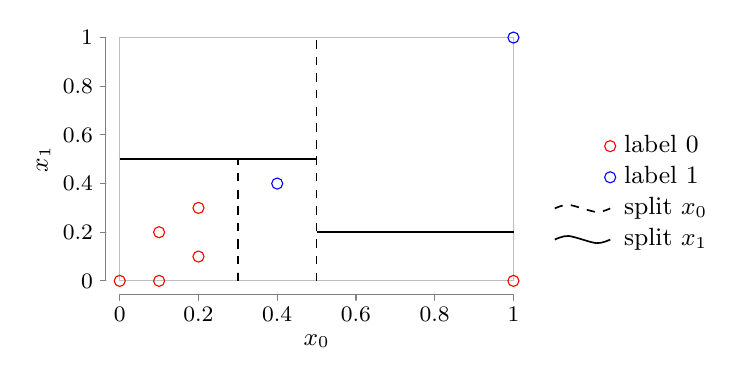
\begin{tikzpicture}
  \datavisualization[
    scientific axes = clean,
    x axis={label={$x_0$}},
    y axis={label={$x_1$}},
    visualize as smooth line/.list={
      split0,split1,split2,split3
    },
    visualize as scatter/.list={0,1},
    0={label in legend={text=label 0},
      style={mark=o, visualizer color=red}},
    1={label in legend={text=label 1},
      style={mark=o, visualizer color=blue}},
    split0={label in legend={text=split $x_0$},
      style={dashed}},
    split1={label in legend={text=split $x_1$}},
    split3={style={dashed}},
  ]
  data {
    x,  y,  set
    0,  0,  0
    0.1,0,  0
    0.2,0.1,0
    0.2,0.3,0
    0.1,0.2,0
    1,  0,  0
    0.4,0.4,1
    1,  1,  1
    0.5,0,  split0
    0.5,1,  split0
    0,  0.5,split1
    0.5,0.5,split1
    0.5,0.2,split2
    1,  0.2,split2
    0.3,0,  split3
    0.3,0.5,split3
  };
\end{tikzpicture}

    \caption{Scatterplot showing the observations and the
      splits done by the FIT operation.}
    \label{fig:scatter_example}
  \end{subfigure}
  \begin{subfigure}[b]{\textwidth}
    \centering
    \scalebox{0.9}{\def\Node#1#2{
  \node[
    rectangle split,
    rectangle split parts=3,
    rectangle split horizontal,
    draw
  ] (#1) {#2\nodepart{two}\nodepart{three}};
}
\def\NodeR#1#2#3{
  \node[
    rectangle split,
    rectangle split parts=3,
    rectangle split horizontal,
    draw,
    #3
  ] (#1) {#2};
}
\def\LeafR#1#2#3{
  \node[
    rectangle split,
    rectangle split parts=3,
    rectangle split horizontal,
    rounded corners,
    draw,
    #3
   ] (#1) {#2};
}
\def\l#1#2{
  \draw[->] ($(#1.two split)!.5!(#1.text split)$)
    |- ($(#1.south)!.5!(#2.north)$) -| (#2.north);
}
\def\r#1#2{
  \draw[->] ($(#1.two split)!.5!(#1.east)$)
    |- ($(#1.south)!.5!(#2.north)$) -| (#2.north);
}
\def\D#1#2#3{
  \matrix[
    ampersand replacement=\&,
    matrix of nodes,
    left delimiter={[},
    right delimiter={]},
    outer ysep=3pt,
    #2
  ] (#1) {#3};
}

\begin{tikzpicture}[
  every left delimiter/.style={xshift=2ex},
  every right delimiter/.style={xshift=-2ex},
]
  % for margin
  \node at(0,1) {};

  \Node{root}{0.5}
    \NodeR{al}{0.5}{below left=0.5 and 2 of root}
      \NodeR{bl}{0.3}{below left=0.5 of al}
        \LeafR{lb}{true}{below left=0.5 and 0.1 of bl}
          \D{lbx}{below left=0.5 and -.75 of lb} {
            0   \& 0   \\
            0.1 \& 0   \\
            0.2 \& 0.1 \\
            0.2 \& 0.3 \\
            0.1 \& 0.2 \\
          }
          \D{lby}{below right=0.5 and .15 of lb} {
            0 \\
            0 \\
            0 \\
            0 \\
            0 \\
          }
        \LeafR{lc}{false}{below right=.5 and 0.1 of bl}
          \D{lcx}{below left=0.5 and -.75 of lc} {
            0.4 \& 0.4 \\
          }
          \D{lcy}{below right=.5 and .15 of lc}{
            1 \\
          }
      \LeafR{la}{false}{below right=0.5 of al}
        \D{lax}{below left=.3 and -.75 of la}{
          \textcolor{white}{1} \&
          \textcolor{white}{1}\\
        }
        \D{lay}{below right=.3 and .15 of la}{
          \textcolor{white}{1}\\
        }
    \NodeR{ar}{0.2}{below right=0.5 and 2 of root}
      \LeafR{ld}{false}{below left=0.5 of ar}
        \D{ldx}{below left=.3 and -.75 of ld} {
          1 \& 0 \\
        }
        \D{ldy}{below right=.3 and .15 of ld} {0 \\}
      \LeafR{le}{false}{below right=0.5 of ar}
        \D{lex}{below left=.3 and -.75 of le} {
          1 \& 1 \\
        }
        \D{ley}{below right=.3 and .15 of le} {1 \\}

  \l{root}{al}
    \l{al}{bl}
      \l{bl}{lb}
        \l{lb}{lbx}
        \r{lb}{lby}
      \r{bl}{lc}
        \l{lc}{lcx}
        \r{lc}{lcy}
    \r{al}{la}
      \l{la}{lax}
      \r{la}{lay}
  \r{root}{ar}
    \l{ar}{ld}
      \l{ld}{ldx}
      \r{ld}{ldy}
    \r{ar}{le}
      \l{le}{lex}
      \r{le}{ley}

  \node[
    rectangle split,
    rectangle split parts=3,
    rectangle split horizontal,
    draw,
    below=3.5 of ar
  ] (nd) {};
  \node[right] at (nd.east) {Node};

  \node[
    rectangle split,
    rectangle split parts=3,
    rectangle split horizontal,
    rounded corners,
    draw,
    below=.5 of nd
   ] (lf) {};
   \node[right] at (lf.east) {Leaf};
\end{tikzpicture}
}
    \caption{The structure of the Tree generated by FIT.}
    \label{fig:tree_example}
  \end{subfigure}
  \caption{Example of FIT applied to the dataset seen in
    Figure~\ref{fig:scatter_example}. $\gamma$ simply
    computes the probability of each label in $y$ and
    returns a function returning the label with the
    maximum probability and as loss one minus the maximum
    probability. The thresholds are: $\tau_l = 1$,
    $\tau_{|X|} = 2$. $\tau_h$ can be any integer above
    2.
  }
  \label{fig:fit_example}
\end{figure*}


\subsection{The PREDICT operation}

The PREDICT operation traverses a Tree until it encounters
a Leaf. If the Leaf is active a label to a provided
observation $x$ is returned by the predictor
property of the Leaf, otherwise $\Lambda$ is returned.

$\Lambda$ must not be an element of the label set.

\begin{algorithm}
  \caption{: PREDICT($\Theta, x, h$)}%
  \label{alg:pred}
  Inputs:

    \begin{tabu}{llX}
    $\Theta$ &$-$ &a Tree node; initially pointing to the
      root of the Tree,\\
    $x$ &$-$ &an observation,\\
    $h$ &$-$ &height of the Tree; initially $h = 0$
    \end{tabu}

  Output: the predicted label or $\Lambda$

  \noindent\rule{\linewidth}{0.4pt}

  \begin{algorithmic}[1]
    \IF{TYPE($\Theta$) is Node}
      \STATE dimension $\leftarrow h$ mod $|x|$
      \IF{$x[dimension] \leq \Theta$.split}
        \STATE PREDICT($\Theta$.left, $x$, $h + 1$)
      \ELSE
        \STATE PREDICT($\Theta$.right, $x$, $h + 1$)
      \ENDIF
    \ELSIF{$\Theta$.active}
      \RETURN $\Theta$.predictor($x$)
    \ELSE
      \RETURN $\Lambda$
    \ENDIF
  \end{algorithmic}
\end{algorithm}



\section{Possible additional features}
\label{sec:features}

There are some possible features and optimizations to the
PCF which were not discussed in the previous Sections.
Again it should be noted that these features and
optimizations are yet untested (see Section~%
\ref{sec:intro}).

The proposed features are:

\begin{enumerate}

  \item Weighing partitions.

  \item Compressing a Tree after FIT.

  \item Select k best or reducing $N$ in another way.

  \item Choosing the dimension a Node has randomly rather
        than cyclic (see Section~\ref{subsec:fit}).

  \item Add a rotation matrix to every Tree.

  \item A second, more light-weight variant of the PCF
        reducing the memory usage, depending on $\gamma$.

\end{enumerate}

The first feature would be to weigh partitions. As of
right now, the PCF's PREDICT operation determines $l_{max}$
as the label predicted most (Algorithm~\ref{alg:pcf_pred},
line 5).

This could be further refined with weighing each partition
based on two properties: (\romannumeral 1) the amount
of observations a partition contains and (\romannumeral 2)
its volume. This would result in a weight determined as:
\begin{align}
  \text{weight(partition)} = \frac{|\text{partition}.X|}
  {V(\text{partition})}.
\end{align}
A partition with a lot of observations and a small
volume would have a higher weight than one with a small
amount of observations and a high volume, further
increasing the probability that the label predicted by the
partition with the higher weight is determined as
$l_{max}$. So instead of just counting each label predicted
and returning the one predicted most, the weight of each
prediction is summed and the label with the highest sum
will be returned by PREDICT as $l_{max}$.

The second optimization is compressing a Tree after FIT.
If a Node has two inactive Leaves as children the Node is
unnecessary since either way $\Lambda$ is returned. The
Node could be transformed into an inactive Leaf, reducing
the path length of the branch by one and decreasing the
amount of nodes by two, which decreases the size of the
Tree and therefore the time complexity of PREDICT.

Another feature would be to reduce the amount of Trees $N$
after FIT, removing Trees with little active partitions
from the PCF instance, decreasing the time complexity
of PREDICT.

Two features inspired by methods used in the Approximate
Nearest Neighbor Search are (\romannumeral 1) choosing the
splitting dimension --- like the splitting value --- at
random rather than cyclic (see Section~\ref{subsec:fit})
and (\romannumeral 2) also rotating the data for each Tree
instance.\cite[pages 17 - 27]{anns} This further increases
the possibility of having Trees with different structures
and therefore partitions.\cite[page 24]{anns}

In Section~\ref{sec:application} and in Figure~%
\ref{fig:fit_example} a very simple classifier is returned
by $\gamma$. It only computes the probability for each
label and returns the label with the highest probability
(see Figure~\ref{fig:fit_example}).

A classifier like that does not need to know where the
observations are in the partition which makes it
unnecessary to keep them in a Leaf node as $X$ and $y$
(see Algorithm~\ref{alg:fit}). Instead a dictionary with
every label from the label space where each label is mapped
to the amount of observations inside the partition having
the particular label is enough. A possible feature would be
to provide a second variant of the PCF which passes this
dictionary instead of the observations to $\gamma$,
decreasing the complexity of the PCF for classifiers which
do not need to know where each observations lays inside the
partition.


\section{Conclusion}
\label{sec:conclusion}

%This paper provides an early Proof of Concept of the
%Partial Classification Forest. It describes the core
%structures and methods of the PCF and shows its use on an
%artificial problem designed to display the use of it over
%other classifiers which take the whole feature space to
%. There is yet much to
%test, discover and first and foremost to implement.

\bibliography{pcf}

\end{document}
